% Usage: knitr slide


\def\apacue{1}
\chapter{Serial Data}
\section{Introduction}\soundm{serial-1}\ipacue
Serial data, also called longitudinal data, repeated measures, or
panel data,
present a special challenge in that the response variable is
multivariate, and that the responses measured at different times (or
other conditions such as doses) but on the same subject are correlated
with each other.  One expects correlations between two
measurements measured closer together will exceed correlations for two
distant measurements on the same subject.  Analyzing the repeated
measurements just as
though they were independent measurements falsely inflates the sample
size and results in a failure to preserve type~I error and confidence
interval coverage.  For example, having three measurements on 10
subjects results in 30 measurements, but depending on the correlations
among the three measurements within subject, the effective sample size
might be 16, for example.  In other words, the statistical information
for collecting 3 measurements on each of 10 subjects might provide the
same statistical information and power as having one measurement on
each of 16 subjects.  The statistical information would however be less than
that from 30 subjects measured once, if the intra-subject correlation
exceeds zero.

The most common problems in analyzing serial data are
\be
\item treating repeated measurements per subject as if they were from separate subjects
\item using two-way ANOVA as if different measurement times corresponded to different groups of subjects
\item using repeated measures ANOVA which assumes that the correlation between any two points within subject is the same regardless of how far apart the measures were timed
\item analyzing more than 3 time points as if time is a categorical rather than a continuous variable
 \bi
 \item multiplicity problem
 \item analyses at different times may be inconsistent since times are not connected
 \item loss of power by not jointly analyzing the serial data
 \ei
\ee


\section{Analysis Options}\ipacue
There are several overall approaches to the analysis of serial
measurements.  Some of the older approaches such as multiple $t$-tests
and repeated measures ANOVA are
now considered obsolete because of the availability of better methods that are
more flexible and robust\footnote{Repeated measures ANOVA makes stringent assumptions and requires complex adjustments for within-subject correlation.}.
Separate $t$-tests at each time point do not make good use of
available information, use an inefficient estimate of $\sigma^2$, do
not interpolate time points, and have multiple comparison problems.
Since a multiplicity adjustment for multiple correlated $t$-tests is
not model-based, the resulting confidence intervals and $P$-values
are conservative.  To preserve type I error, one always must sacrifice
type II error, but in this case the sacrifice is too severe.
In addition, investigators are frequently confused by the $t$-test being
``significant'' at one time point and not at another, and make the
unwarranted claim that the treatment is effective only at the first
time.  Besides not recognizing the \emph{absence of evidence is not evidence for absence} problem, the investigator can be mislead by
increased variability in response at the second time point driving
the $t$ ratio towards zero.  This variability may not even be real but
may reflect instability in estimating $\sigma$ separately at each time
point.

Especially when there are more than three unique measurement times, it is advisable to model time as a continuous variable.  When estimation of the time-response profile is of central importance, that may be all that's needed.  When comparing time-response profiles (e.g., comparing two treatments) one needs to carefully consider the characteristics of the profiles that should be tested, i.e., where the type I and II errors should be directed, for example
\bi
\item difference in slope
\item difference in area under the curve
\item difference in mean response at the last planned measurement time
\item difference in mean curves at \emph{any} time, i.e., whether the curves have different heights or shapes anywhere
\ei
The first 3 are 1 d.f.\ tests, and the last is a 2 d.f.\ test if linearity is assumed, and $> 2$ d.f.\ if fitting a polynomial or spline function.

\subsection{Joint Multivariate Models}\ipacue
This is the formal fully-specified statistical model approach whereby
a likelihood function is formed and maximized.  This handles highly
imbalanced data, e.g., one subject having one measurement and another
having 100.  It is also the most robust approach to non-random subject
dropouts.  These two advantages come from the fact that full
likelihood models ``know'' exactly how observations from the same
subject are connected to each other.

Examples of full likelihood-based models include
generalized least squares, mixed effects models, and Bayesian hierarchical
models.  Generalized least
squares only handles continuous $Y$ and assumes multivariate
normality.  It does not allow different subjects to have different
slopes.  But it is easy to specify and interpret, to have its assumptions
checked, and it runs faster.
Mixed effects models can handle multiple hierarchical levels (e.g.,
state/hospital/patient) and random slopes whereby subjects can
have different trajectories.  Mixed effects models can be generalized
to binary and other endpoints but lose their full likelihood status
somewhat when these extensions are used, unless a Bayesian approach is used.

\bi
\item Mixed effects model have random effects (random intercepts and possibly also random slopes or random shapes) for subjects
\item These allow estimation of the trajectory for an individual subject
\item When the interest is instead on group-level effects (e.g., average difference between treatments, over subjects), GLS squares models may be more appropriate
\item The generalization of GLS to non-normally distributed $Y$ is \emph{marginalized models} (marginalized over subject-level effects)
\ei

Generalized least squares, formerly called growth curve models, is the
oldest approach and has excellent performance when $Y$ is
conditionally normally distributed.

\subsection{GEE}\ipacue
\emph{Generalized estimating equations} is usually based on a working
independence model whereby ordinary univariate regressions are fitted on a
combined dataset as if all observations are uncorrelated, and then an
after-the-fit correction for intra-cluster
correlation is done using the cluster sandwich covariance estimator or the
cluster bootstrap.  GEE is very non-robust to non-random subject dropout; it
assumes missing response values are missing completely at random.  It
may also require large sample sizes for
$P$-values and confidence intervals to be accurate.  An advantage of GEE is
that it extends easily to every type of response variable, including binary,
ordinal, polytomous, and time-to-event responses.

\subsection{Summary Measures}\soundm{serial-2}\ipacue
A simple and frequently effective approach is to summarize the serial
measures from each subject using one or two measures, then to analyze
these measures using traditional statistical methods that capitalize
on the summary measures being independent for different subjects.
This has been called
\be
\item Two-stage derived variable analysis~\cite{diggle-longit}
\item Response feature analysis~\cite{dupmod}
\item Longitudinal analysis through summary measures~\cite{mat90ana}
\ee
An excellent overview may be found in \citet{mat90ana},
\citet{dupmod} (Chapter 11), and \citet{sen00rep}.

Frequently chosen summary measures include the area under the
time-response curve, slope, intercept, and consideration of multiple
features simultaneously, e.g., intercept, coefficient of time,
coefficient of time squared when fitting each subject's data with a
quadratic equation.  This allows detailed analyses of curve shapes.

\section{Case Study}
\subsection{Data and Summary Measures}\soundm{serial-3}\ipacue
Consider the isoproterenol dose-response analysis of \citet{dupmod} of
the original data from Lang\footnote{CC Lang~\etal\ NEJM 333:155-60, 1995}.  Twenty two normotensive men were studied, 9 of
them black and 13 white.  Blood flow was measured before the drug was
given, and at escalating doses of isoproterenol.  Most subjects had 7
measurements, and these are not independent.
\begin{Schunk}
\begin{Sinput}
require(Hmisc)
require(data.table)   # elegant handling of aggregation
\end{Sinput}
\begin{Sinput}
require(ggplot2)
d <- csv.get('https://hbiostat.org/data/repo/11.2.Long.Isoproterenol.csv')
d <- upData(d, keep=c('id', 'dose', 'race', 'fbf'),
            race  =factor(race, 1:2, c('white', 'black')),
            labels=c(fbf='Forearm Blood Flow'),
            units=c(fbf='ml/min/dl'))
\end{Sinput}
\begin{Soutput}
Input object size:	 13168 bytes;	 8 variables	 154 observations
Modified variable	race
Kept variables	id,dose,race,fbf
New object size:	6496 bytes;	4 variables	154 observations
\end{Soutput}
\begin{Sinput}
d <- data.table(d)
setkey(d, id, race)
\end{Sinput}
\end{Schunk}

\begin{Schunk}
\begin{Sinput}
# Fit subject-by-subject spline fits and either return the coefficients,
# the estimated area under the curve from [0,400], or evaluate each
# subject's fitted curve over a regular grid of 150 doses
# Area under curve is divided by 400 to get a mean function
require(rms)
\end{Sinput}
\begin{Sinput}
options(prType='latex')
g <- function(x, y, what=c('curve', 'coef', 'area')) {
  what <- match.arg(what)   # 'curve' is default
  knots <- c(20, 60, 150)
  f <- ols(y ~ rcs(x, knots))
  xs <- seq(0, 400, length=150)
  switch(what,
         coef = {k <- coef(f)
                 list(b0 = k[1], b1=k[2], b2=k[3])},
         curve= {x <- seq(0, 400, length=150)
                 list(dose=xs, fbf=predict(f, data.frame(x=xs)))},
         area = {antiDeriv = rcsplineFunction(knots, coef(f),
                   type='integral')
                 list(dose  = 400, fbf=y[x == 400],
                      area  = antiDeriv(400) / 400,
                      tarea = areat(x, y) / 400)} )
}
# Function to use trapezoidal rule to compute area under the curve
areat <- function(x, y) {
  i <- ! is.na(x + y)
  x <- x[i]; y <- y[i]
  i <- order(x)
  x <- x[i]; y <- y[i]
  if(! any(x == 400)) NA else
  sum(diff(x) * (y[-1] + y[-length(y)]))/2
}

w <- d[, j=g(dose, fbf), by = list(id, race)]   # uses data.table package
a <- d[, j=g(dose, fbf, what='area'), by = list(id, race)]

ggplot(d, aes(x=dose, y=fbf, color=factor(id))) +   # Fig. (*\ref{fig:serial-spag}\ipacue*)
       geom_line() + geom_line(data=w, alpha=0.25) +
       geom_text(aes(label = round(area,1)), data=a, size=2.5,
                 position=position_dodge(width=50)) +
       xlab('Dose') + ylab(label(d$fbf, units=TRUE, plot=TRUE)) +
       facet_grid(~ race) +
       guides(color=FALSE)
\end{Sinput}
\begin{figure}[htbp]

\centerline{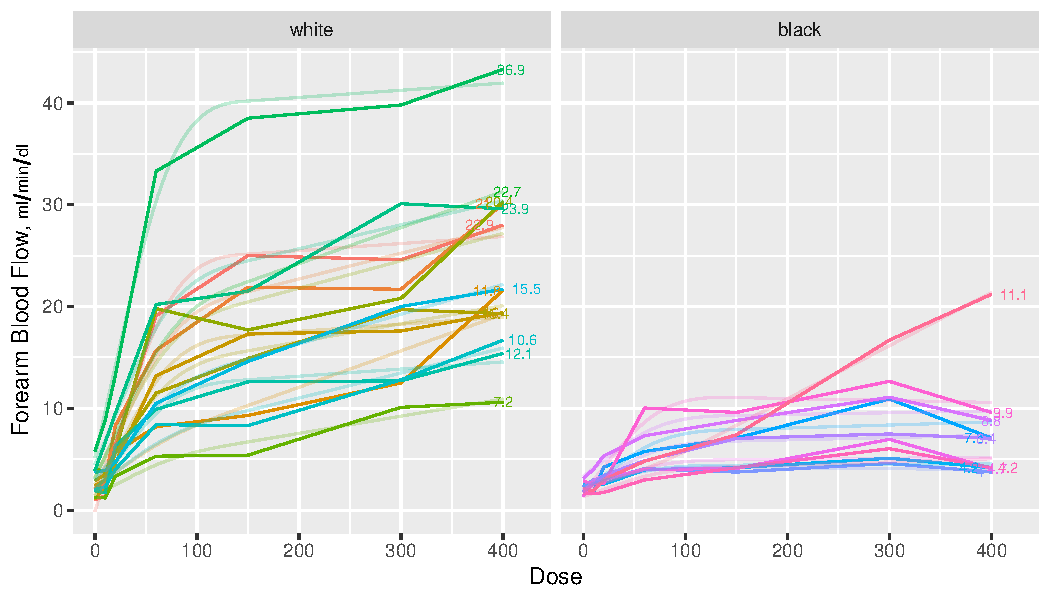
\includegraphics[width=\maxwidth]{serial-spag-1} }

\caption[Spaghetti plots for isoproterenol data]{Spaghetti plots for isoproterenol data showing raw data stratified by race.  Next to each curve is the area under the curve divided by 400 to estimate the mean response function.  The area is computed analytically from a restricted cubic spline function fitted separately to each subject's dose-response curve.  Shadowing the raw data are faint lines depicting spline fits for each subject}\label{fig:serial-spag}
\end{figure}
\end{Schunk}

\begin{Schunk}
\begin{Sinput}
ggplot(a, aes(x=tarea, y=area, color=race)) + geom_point() +
  geom_abline(col=gray(.8)) +
  xlab('Area by Trapezoidal Rule / 400') +
  ylab('Area by Spline Fit / 400')          # Fig. (*\ref{fig:serial-auctwo}\ipacue*)
\end{Sinput}
\begin{figure}[htbp]

\centerline{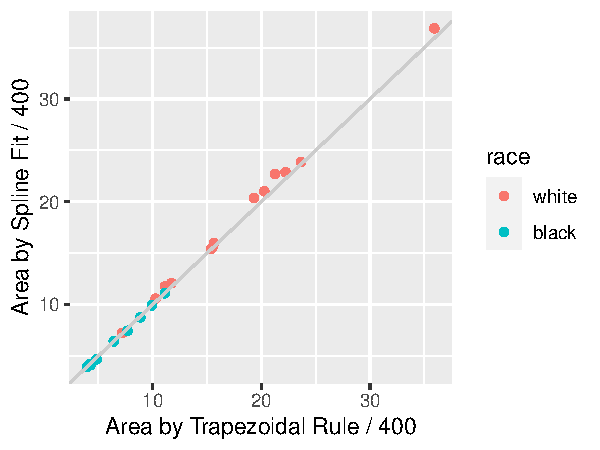
\includegraphics[width=\maxwidth]{serial-auctwo-1} }

\caption[AUC by curve fitting and by trapezoidal rule]{AUC by curve fitting and by trapezoidal rule}\label{fig:serial-auctwo}
\end{figure}
\end{Schunk}
When a subject's dose (or time) span includes the minimum and maximum values
over all subjects, one can use the trapezoidal rule to estimate the area under
the response curve empirically.  When interior points are missing, linear
interpolation is used.  The spline fits use nonlinear interpolation, which is
slightly better, as is the spline function's assumption of continuity in the
slope.  Figure~\ref{fig:serial-auctwo} compares the area under the curve (divided
by 400 to estimate the mean response) estimated using the the two methods.
Agreement is excellent.  In this example, the principle advantage of the spline
approach is that slope and shape parameters are estimated in the process, and
these parameters may be tested separately for association with group (here,
race).  For example, one may test whether slopes differ across groups, and
whether the means, curvatures, or inflection points differ.  One could
also compare AUC from a sub-interval of $X$.
\begin{Schunk}
\begin{Sinput}
ggplot(a, aes(x=race, y=area)) +    # Fig. (*\ref{fig:serial-auc}\ipacue*)
  geom_boxplot(alpha=.5, width=.25) + geom_point() + coord_flip() +
  ylab(expression(paste('Mean Forearm Blood Flow,  ', scriptstyle(ml/min/dl))))
\end{Sinput}
\begin{figure}[htbp]

\centerline{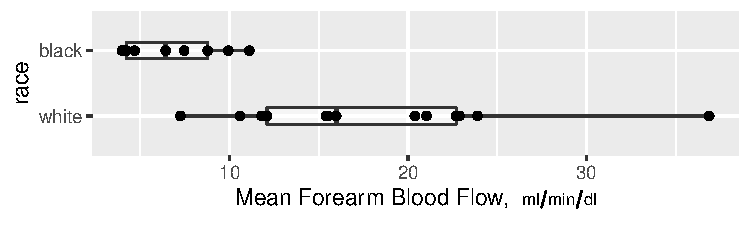
\includegraphics[width=\maxwidth]{serial-auc-1} }

\caption[Mean blood flow by race]{Mean blood flow computed from the areas under the spline curves, stratified by race, along with box plots}\label{fig:serial-auc}
\end{figure}
\end{Schunk}
%\clearpage

\subsection{Nonparametric Test of Race Differences in AUC}\soundm{serial-4}\ipacue
A minimal-assumption approach to testing for differences in
isoproterenol dose-response between races is to apply the Wilcoxon
test to the normalized AUCs (mean response functions).
\begin{Schunk}
\begin{Sinput}
wilcox.test(area ~ race, data=a, conf.int=TRUE)
\end{Sinput}
\begin{Soutput}

	Wilcoxon rank sum exact test

data:  area by race
W = 112, p-value = 7.639e-05
alternative hypothesis: true location shift is not equal to 0
95 percent confidence interval:
  5.670113 16.348121
sample estimates:
difference in location 
              11.25836 
\end{Soutput}
\end{Schunk}
There is strong evidence that the mean response is greater for whites.

\subsection{Nonparametric Test of General Curve Differences}\ipacue
\citet{obr88com} proposed a method for using logistic regression to
turn the Hotelling $T^2$ test on its side.  The Hotelling test is the
multivariate analog of the two-sample $t$-test, and can be used to
test simultaneously such things as whether a treatment modifies either
systolic or diastolic blood pressure.  O'Brien's idea was to test
whether systolic or diastolic blood pressure (or both) can predict
which treatment was given.  Here we use the idea to test for race
differences in the shape of the dose-response curves.  We do this by
predicting race from a 3-predictor model---one containing the intercept, the next the coefficient of the linear dose effect and the third the coefficient of the nonlinear restricted cubic spline term (differences in cubes).
These coefficients were estimated
using ordinary least squares in separately predicting each subject's relationship
between dose and forearm blood flow.
\begin{Schunk}
\begin{Sinput}
h <- d[, j=g(dose, fbf, what='coef'), by = list(id, race)]
h
\end{Sinput}
\begin{Soutput}
    id  race         b0         b1          b2
 1:  1 white -0.1264763 0.32310327 -0.34253352
 2:  2 white  2.1147707 0.22798336 -0.21959542
 3:  3 white  2.3378721 0.06927717 -0.03625384
 4:  4 white  1.4822502 0.19837740 -0.20727584
 5:  5 white  2.5366751 0.15399740 -0.14756999
 6:  6 white  3.2117187 0.19910942 -0.18650561
 7:  7 white  1.4264366 0.05261565 -0.03871545
 8:  8 white  3.0999999 0.21833887 -0.19813457
 9:  9 white  5.1507764 0.45026617 -0.48013920
10: 10 white  4.4778127 0.23853904 -0.23289815
11: 11 white  1.9052885 0.13548226 -0.13917910
12: 12 white  2.1828176 0.07558431 -0.05524955
13: 13 white  2.9318982 0.12776900 -0.10679867
14: 14 black  2.3336099 0.02679742 -0.02856275
15: 15 black  1.8356227 0.07652884 -0.07972036
16: 16 black  2.5342537 0.02290717 -0.02585081
17: 17 black  2.0254606 0.06002835 -0.06261969
18: 18 black  3.3279080 0.07620477 -0.08062536
19: 19 black  1.9308650 0.03844018 -0.04060065
20: 20 black  1.7263259 0.12358392 -0.13595538
21: 21 black  1.3215502 0.03528716 -0.03480467
22: 22 black  2.0828281 0.03143768  0.02251155
    id  race         b0         b1          b2
\end{Soutput}
\end{Schunk}
\begin{Sinput}
f <- lrm(race ~ b0 + b1 + b2, data=h, x=TRUE, y=TRUE)
f
\end{Sinput}

 \noindent \textbf{Logistic Regression Model}
 
 \begin{verbatim}
 lrm(formula = race ~ b0 + b1 + b2, data = h, x = TRUE, y = TRUE)
 \end{verbatim}
 
 {\fontfamily{phv}\selectfont \begin{center}\begin{tabular}{|c|c|c|c|}\hline
&Model Likelihood&Discrimination&Rank Discrim.\\
&Ratio Test&Indexes&Indexes\\\hline
Obs~\hfill 22&LR $\chi^{2}$~\hfill 19.73&$R^{2}$~\hfill 0.798&$C$~\hfill 0.957\\
~~white~\hfill 13&d.f.~\hfill 3&$g$~\hfill 6.783&$D_{xy}$~\hfill 0.915\\
~~black~\hfill 9&Pr$(>\chi^{2})$~\hfill 0.0002&$g_{r}$~\hfill 882.952&$\gamma$~\hfill 0.915\\
$\max|\frac{\partial\log L}{\partial \beta}|$~\hfill $8\!\times\!10^{-7}$&&$g_{p}$~\hfill 0.471&$\tau_{a}$~\hfill 0.463\\
&&Brier~\hfill 0.080&\\
\hline
\end{tabular}
\end{center}}
 
 %latex.default(U, file = "", first.hline.double = FALSE, table = FALSE,     longtable = TRUE, lines.page = lines.page, col.just = rep("r",         ncol(U)), rowlabel = "", already.math.col.names = TRUE,     append = TRUE)%
 \setlongtables\begin{longtable}{lrrrr}\hline
 \multicolumn{1}{l}{}&\multicolumn{1}{c}{$\hat{\beta}$}&\multicolumn{1}{c}{S.E.}&\multicolumn{1}{c}{Wald $Z$}&\multicolumn{1}{c}{Pr$(>|Z|)$}\tabularnewline
 \hline
 \endhead
 \hline
 \endfoot
 Intercept&~   3.6618~&~ 4.1003~& 0.89&0.3718\tabularnewline
 b0&~   1.3875~&~ 2.5266~& 0.55&0.5829\tabularnewline
 b1&~-165.3481~&~92.7864~&-1.78&0.0747\tabularnewline
 b2&~-101.1667~&~63.1549~&-1.60&0.1092\tabularnewline
 \hline
 \end{longtable}
 \addtocounter{table}{-1}

The likelihood ratio $\chi^{2}_{3}=19.73$ has $P=0.0002$ \ipacue
indicating strong evidence that the races have different averages,
slopes, or shapes of the dose-response curves.  The $c$-index of 0.957
indicates nearly perfect ability to separate the races on the basis of three
curve characteristics (although the sample size is small).  We can use
the bootstrap to get an overfitting-corrected index.
\begin{Sinput}
set.seed(2)
v <- validate(f, B=1000)
\end{Sinput}

Divergence or singularity in 271 samples
\begin{Sinput}
latex(v)
\end{Sinput}
\Needspace{2in}
\begin{center}\normalsize
%latex.default(unclass(x), cdec = cdec, rowlabel = "Index", title = title,     caption = if (table.env) caption, table.env = table.env,     file = file, append = TRUE, center = "none", extracolsize = extracolsize,     ...)%
\begin{tabular}{lrrrrrr}
\hline\hline
\multicolumn{1}{l}{Index}&\multicolumn{1}{c}{Original}&\multicolumn{1}{c}{Training}&\multicolumn{1}{c}{Test}&\multicolumn{1}{c}{Optimism}&\multicolumn{1}{c}{Corrected}&\multicolumn{1}{c}{$n$}\tabularnewline
&\multicolumn{1}{c}{{\normalsize Sample}}&\multicolumn{1}{c}{{\normalsize Sample}}&\multicolumn{1}{c}{{\normalsize Sample}}&&\multicolumn{1}{c}{{\normalsize Index}}&\tabularnewline
\hline
$D_{xy}$&$ 0.9145$&$ 0.9589$&$ 0.8423$&$ 0.1166$&$  0.7980$&$729$\tabularnewline
$R^{2}$&$ 0.7985$&$ 0.9096$&$ 0.6617$&$ 0.2479$&$  0.5506$&$729$\tabularnewline
Intercept&$ 0.0000$&$ 0.0000$&$ 0.1150$&$-0.1150$&$  0.1150$&$729$\tabularnewline
Slope&$ 1.0000$&$ 1.0000$&$ 0.4259$&$ 0.5741$&$  0.4259$&$729$\tabularnewline
$E_{\max}$&$ 0.0000$&$ 0.0000$&$ 0.2056$&$ 0.2056$&$  0.2056$&$729$\tabularnewline
$D$&$ 0.8513$&$ 1.0728$&$ 0.6434$&$ 0.4294$&$  0.4219$&$729$\tabularnewline
$U$&$-0.0909$&$-0.0909$&$ 2.6080$&$-2.6989$&$  2.6080$&$729$\tabularnewline
$Q$&$ 0.9422$&$ 1.1637$&$-1.9646$&$ 3.1283$&$ -2.1861$&$729$\tabularnewline
$B$&$ 0.0803$&$ 0.0310$&$ 0.0773$&$-0.0463$&$  0.1266$&$729$\tabularnewline
$g$&$ 6.7833$&$23.8206$&$ 4.4145$&$19.4061$&$-12.6228$&$729$\tabularnewline
$g_{p}$&$ 0.4712$&$ 0.4629$&$ 0.4255$&$ 0.0373$&$  0.4339$&$729$\tabularnewline
\hline
\end{tabular}
\end{center}

The overfitting-corrected $c$-index is $c = \frac{D_{xy} + 1}{2}$ = 0.9.

\subsection{Model-Based Analysis: Generalized Least Squares}\soundm{serial-5}\ipacue
Generalized least squares (GLS) is the first generalization of ordinary
least squares (multiple linear regression).  It is described in detail
in \emph{Regression Modeling Strategies} Chapter~7 where a
comprehensive case study is presented.  The assumptions of GLS are
\bi
\item All the usual assumptions about the right-hand-side of the model
  related to transformations of $X$ and interactions
\item Residuals have a normal distribution
\item Residuals have constant variance vs.\ $\hat{Y}$ or any $X$ (but
  the G in GLS also refers to allowing variances to change across $X$)
\item The multivariate responses have a multivariate normal
  distribution conditional on $X$
\item The correlation structure of the conditional multivariate
  distribution is correctly specified
\ei
With fully specified serial data models such as GLS, the fixed effects
of time or dose are modeled just as any other predictor, with the only
difference being that it is the norm to interact the time or dose
effect with treatment or whatever $X$ effect is of interest.  This
allows testing hypotheses such as
\bi
\item Does the treatment effect change over time? (time $\times$
  treatment interaction)
\item Is there a time at which there is a treatment effect? (time
  $\times$ treatment interaction + treatment main effect combined into
  a chunk test)
\item Does the treatment have an effect at time $t$? (difference of
  treatments fixing time at $t$, not assuming difference is constant
  across different $t$)
\ei
In the majority of longitudinal clinical trials, the last hypothesis \ipacue
is the most important, taking $t$ as the end of treatment point.  This
is because one is often interested in where patients ended up, not
just whether the treatment provided temporary relief.

Now consider the isoproterenol dataset and fit a GLS model allowing for
the same nonlinear spline effect of dose as was used above, and
allowing the shapes of curves to be arbitrarily different by race.  We
impose a continuous time AR1 correlation structure on within-subject
responses.  This is the most commonly used correlation structure; it
assumes that the correlation between two points is exponentially
declining as the difference between two times or doses
increases.
We fit the GLS model and examine the equal variance assumption.
\begin{Schunk}
\begin{Sinput}
require(nlme)
\end{Sinput}
\begin{Sinput}
dd <- datadist(d); options(datadist='dd')
a <- Gls(fbf ~ race * rcs(dose, c(20,60,150)), data=d,
         correlation=corCAR1(form = ~ dose | id))
plot(fitted(a), resid(a))   # Fig. (*\ref{fig:serial-glsa}\ipacue*)
\end{Sinput}
\begin{figure}[htbp]

\centerline{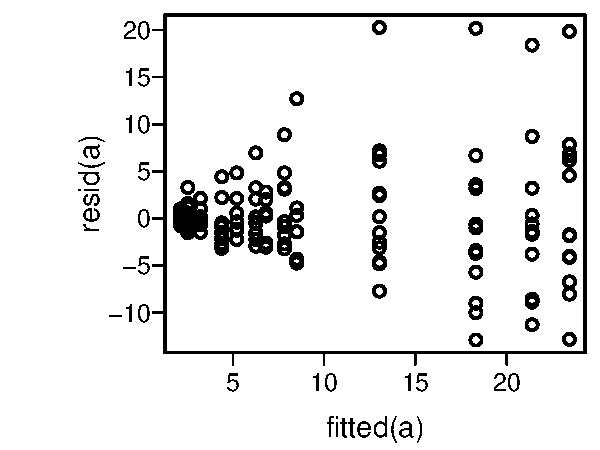
\includegraphics[width=\maxwidth]{serial-glsa-1} }

\caption[Residual plot for generalized least squares fit on untransformed  \co{fbf}]{Residual plot for generalized least squares fit on untransformed  \co{fbf}}\label{fig:serial-glsa}
\end{figure}
\end{Schunk}
The variance of the residuals is clearly increasing with increasing
dose.  Try log transforming both \co{fbf} and dose.  The log
transformation requires a very arbitrary adjustment to dose to handle zeros.
\begin{Sinput}
a <- Gls(log(fbf) ~ race * rcs(log(dose + 1), log(c(20,60,150)+1)), data=d,
         correlation=corCAR1(form = ~ dose | id))
anova(a)
\end{Sinput}
%latex.default(dstats, title = title, caption = if (table.env) caption else NULL,     insert.top = if (length(caption) && !table.env) paste0("\\Needspace{2in}\n",         caption), rowlabel = "", col.just = rep("r", length(sn)),     table.env = table.env, ...)%
\textbf{\Needspace{2in}
Wald Statistics for \texttt{\smaller log(fbf)}}\begin{center}
\begin{tabular}{lrrr}
\hline\hline
\multicolumn{1}{l}{}&\multicolumn{1}{c}{$\chi^{2}$}&\multicolumn{1}{c}{d.f.}&\multicolumn{1}{c}{$P$}\tabularnewline
\hline
race  (Factor+Higher Order Factors)& 99.54&3&\textless 0.0001\tabularnewline
~~\emph{All Interactions}& 19.30&2&\textless 0.0001\tabularnewline
dose  (Factor+Higher Order Factors)&312.10&4&\textless 0.0001\tabularnewline
~~\emph{All Interactions}& 19.30&2&\textless 0.0001\tabularnewline
~~\emph{Nonlinear (Factor+Higher Order Factors)}&  2.01&2&0.3667\tabularnewline
race $\times$ dose  (Factor+Higher Order Factors)& 19.30&2&\textless 0.0001\tabularnewline
~~\emph{Nonlinear}&  0.07&1&0.7969\tabularnewline
~~\emph{Nonlinear Interaction : f(A,B) vs. AB}&  0.07&1&0.7969\tabularnewline
TOTAL NONLINEAR&  2.01&2&0.3667\tabularnewline
TOTAL NONLINEAR + INTERACTION& 21.16&3&\textless 0.0001\tabularnewline
TOTAL&391.48&5&\textless 0.0001\tabularnewline
\hline
\end{tabular}\end{center}

There is little evidence for a nonlinear dose effect on the log scale, \soundm{serial-6}
implying that the underlying model is exponential on the original $X$
and $Y$ scales.  This is consistent with \citet{dupmod}.  Re-fit the
model as linear in the logs.  Before taking this as the final model,
also fit the same model but using a correlation pattern based on time
rather than dose.  Assume equal time spacing during dose escalation. \ipacue
\begin{Schunk}
\begin{Sinput}
a <- Gls(log(fbf) ~ race * log(dose + 1), data=d,
         correlation=corCAR1(form = ~ dose | id))
d$time <- match(d$dose, c(0, 10, 20, 60, 150, 300, 400)) - 1
b <- Gls(log(fbf) ~ race * log(dose + 1), data=d,
         correlation=corCAR1(form = ~ time | id))
AIC(a);AIC(b)
\end{Sinput}
\begin{Soutput}
[1] 231.3731
\end{Soutput}
\begin{Soutput}
[1] 161.3765
\end{Soutput}
\end{Schunk}
Lower AIC is better, so it is clear that time-based correlation
structure is far superior to dose-based.  We will used the second
model for the remainder of the analysis.  But first we check some of
the model assumptions.
\begin{Sinput}
b
\end{Sinput}

 \noindent \textbf{Generalized Least Squares Fit by REML}
 
 \begin{verbatim}
 Gls(model = log(fbf) ~ race * log(dose + 1), data = d, correlation = corCAR1(form = ~time | 
     id))
 \end{verbatim}
 
 {\fontfamily{phv}\selectfont \begin{center}\begin{tabular}{|c|c|}\hline
&\\\hline
Obs~\hfill 150&Log-restricted-likelihood ~\hfill -74.69\\
Clusters~\hfill 22&Model d.f.~\hfill 3\\
$g$~\hfill 0.755&$\sigma$~\hfill 0.5023\\
&d.f.~\hfill 146\\
\hline
\end{tabular}
\end{center}}
 
 %latex.default(U, file = "", first.hline.double = FALSE, table = FALSE,     longtable = TRUE, lines.page = lines.page, col.just = rep("r",         ncol(U)), rowlabel = "", already.math.col.names = TRUE,     append = TRUE)%
 \setlongtables\begin{longtable}{lrrrr}\hline
 \multicolumn{1}{l}{}&\multicolumn{1}{c}{$\hat{\beta}$}&\multicolumn{1}{c}{S.E.}&\multicolumn{1}{c}{$t$}&\multicolumn{1}{c}{Pr$(>|t|)$}\tabularnewline
 \hline
 \endhead
 \hline
 \endfoot
 Intercept&~ 0.9851~&~0.1376~& 7.16&\textless 0.0001\tabularnewline
 race=black&~-0.2182~&~0.2151~&-1.01&0.3120\tabularnewline
 dose&~ 0.3251~&~0.0286~&11.38&\textless 0.0001\tabularnewline
 race=black $\times$ dose&~-0.1421~&~0.0446~&-3.19&0.0018\tabularnewline
 \hline
 \end{longtable}
 \addtocounter{table}{-1}
 \begin{verbatim}
 Correlation Structure: Continuous AR(1)
  Formula: ~time | id 
  Parameter estimate(s):
       Phi 
 0.6886846 
 \end{verbatim}
 
\begin{Sinput}
anova(b)
\end{Sinput}
%latex.default(dstats, title = title, caption = if (table.env) caption else NULL,     insert.top = if (length(caption) && !table.env) paste0("\\Needspace{2in}\n",         caption), rowlabel = "", col.just = rep("r", length(sn)),     table.env = table.env, ...)%
\textbf{\Needspace{2in}
Wald Statistics for \texttt{\smaller log(fbf)}}\begin{center}
\begin{tabular}{lrrr}
\hline\hline
\multicolumn{1}{l}{}&\multicolumn{1}{c}{$\chi^{2}$}&\multicolumn{1}{c}{d.f.}&\multicolumn{1}{c}{$P$}\tabularnewline
\hline
race  (Factor+Higher Order Factors)& 32.45&2&\textless 0.0001\tabularnewline
~~\emph{All Interactions}& 10.16&1&0.0014\tabularnewline
dose  (Factor+Higher Order Factors)&158.11&2&\textless 0.0001\tabularnewline
~~\emph{All Interactions}& 10.16&1&0.0014\tabularnewline
race $\times$ dose  (Factor+Higher Order Factors)& 10.16&1&0.0014\tabularnewline
TOTAL&180.17&3&\textless 0.0001\tabularnewline
\hline
\end{tabular}\end{center}
\begin{Sinput}
w <- data.frame(residual=resid(b), fitted=fitted(b))
p1 <- ggplot(w, aes(x=fitted, y=residual)) + geom_point()
p2 <- ggplot(w, aes(sample=residual)) + stat_qq()
gridExtra::grid.arrange(p1, p2, ncol=2)   # Figure (*\ref{fig:serial-glsc}\ipacue*)
\end{Sinput}
\begin{figure}[htbp]

\centerline{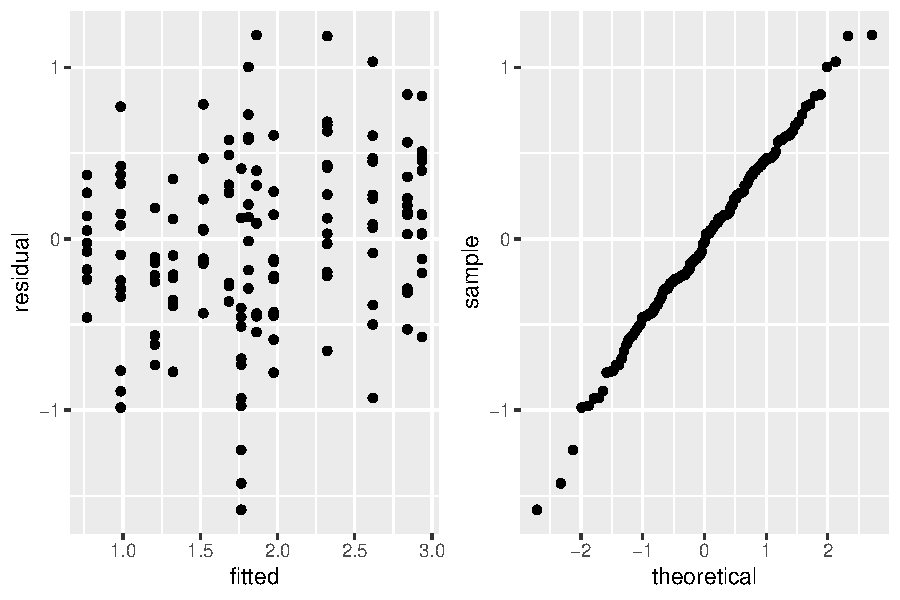
\includegraphics[width=\maxwidth]{serial-glsc-1} }

\caption[Checking assumptions of GLS model]{Checking assumptions of the GLS model that is linear after logging dose and blood flow.  The graph on the right is a QQ-plot to check normality of the residuals from the model, where linearity implies normality.}\label{fig:serial-glsc}
\end{figure}

The test for dose $\times$ race interaction in the above ANOVA summary \ipacue
of Wald statistics shows strong evidence for difference in curve
characteristics across races.  This test agrees in magnitude
with the less parametric approach using the logistic model above.  But
the logistic model also tests for an overall shift in distributions
due to race, and the more efficient test for the combined race main
effect and dose interaction effect from GLS is more significant
with a Wald $\chi^{2}_{2} = 32.45$\footnote{The $\chi^2$ for race with the dose-based correlation structure was a whopping 100 indicating that lack of fit of the correlation structure can have a significant effect on the rest of the GLS model.}. The
estimate of the correlation between two log blood flows measured on
the same subject one time unit apart is 0.69.

The equal variance and normality assumptions appear to be well met as
judged by Figure~\ref{fig:serial-glsc}.

Now estimate the dose-response curves by race, with pointwise \soundm{serial-7}
confidence intervals and simultaneous intervals that allow one to make
statements about the entire curves\footnote{Since the model is linear in log dose there are two parameters involving dose---the dose main effect and the race $\times$ dose interaction effect.  The simultaneous inference adjustment only needs to reflect simultaneity in two dimensions.}.  Anti-log the predicted values to
get predictions on the original blood flow scale.  Anti-logging
predictions from a model that assumes a normal distribution on the
logged values results in estimates of the median response.
\begin{Schunk}
\begin{Sinput}
dos <- seq(0, 400, length=150)
p <- Predict(b, dose=dos, race, fun=exp)
s <- Predict(b, dose=dos, race, fun=exp, conf.type='simultaneous')
ps <- rbind(Pointwise=p, Simultaneous=s)
ggplot(ps, ylab=expression(paste('Median Forearm Blood Flow,  ',
                          scriptstyle(ml/min/dl))))   # Fig. (*\ref{fig:serial-glsd}\ipacue*)
\end{Sinput}
\begin{figure}[htbp]

\centerline{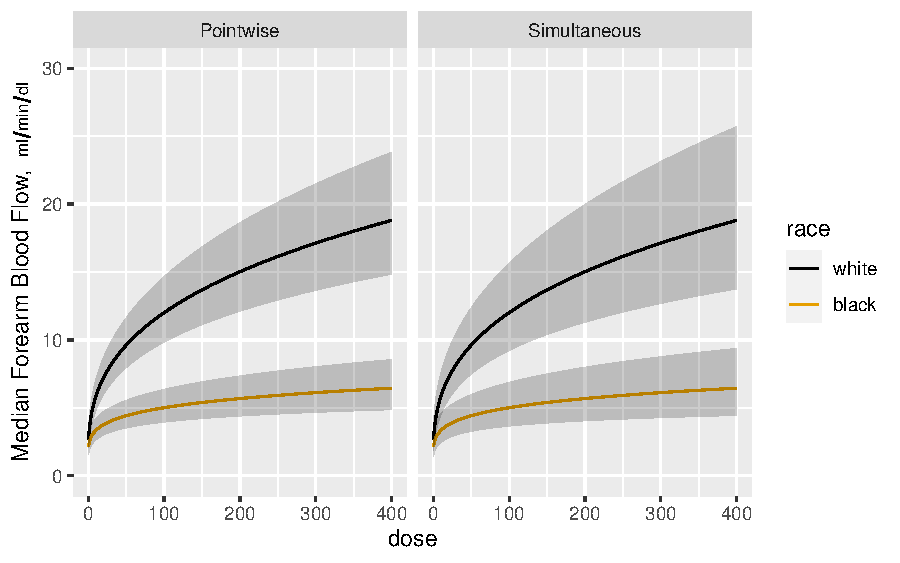
\includegraphics[width=\maxwidth]{serial-glsd-1} }

\caption[Confidence bands for median dose-response curves]{Pointwise and simultaneous confidence bands for median dose-response curves by race}\label{fig:serial-glsd}
\end{figure}
\end{Schunk}
Finally we estimate the white:black fold change (ratio of medians) as
a function of dose with simultaneous confidence bands.
\begin{Schunk}
\begin{Sinput}
k <- contrast(b, list(dose=dos, race='white'),
                 list(dose=dos, race='black'), conf.type='simultaneous')
k <- as.data.frame(k[c('dose', 'Contrast', 'Lower', 'Upper')])
ggplot(k, aes(x=dose, y=exp(Contrast))) + geom_line() +
  geom_ribbon(aes(ymin=exp(Lower), ymax=exp(Upper)), alpha=0.2, linetype=0,
              show_guide=FALSE) +
  geom_hline(yintercept=1, col='red', size=.2) +
  ylab('White:Black Ratio of Median FBF')    # Fig. (*\ref{fig:serial-glse}\ipacue*)
\end{Sinput}
\begin{figure}[htbp]

\centerline{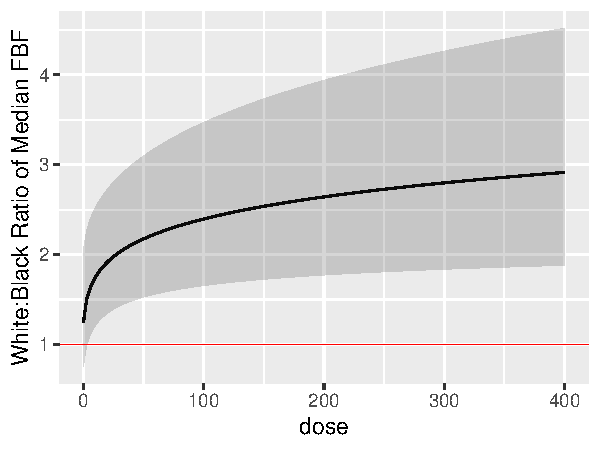
\includegraphics[width=\maxwidth]{serial-glse-1} }

\caption[White:black fold change for median response as a function of dose, with simultaneous confidence band]{White:black fold change for median response as a function of dose, with simultaneous confidence band}\label{fig:serial-glse}
\end{figure}
\end{Schunk}
By comparing the simultaneous confidence binds to the red horizontal
line, one can draw the inference that the dose-response for blacks is
everywhere different than that for whites when the dose exceeds zero.
\def\apacue{0}
